% -*- latex -*-
% FILE: "/home/evmik/jobs/wm/2012_spring_Analog_Electronics_252/midterm_week_5/phys252_midterm_2012.v2.tex"
% LAST MODIFICATION: "Mon, 27 Feb 2012 10:19:43 -0500 (evmik)"
% (C) 2009 by Eugeniy Mikhailov, <evgmik@gmail.com>
% $Id:$

\documentclass[letterpaper,addpoints,answers]{exam}
\usepackage{graphicx}

\newcommand{\hide}[1]{%
}

\begin{document}
%\pagestyle{headandfoot}
%\lhead{
	%\large\bfseries Physics 107\\ 
	%Midterm Exam, June 15, 2009
%}
%\chead{}
%\rhead{
	%\large\bfseries Name:\enspace\makebox[2in]{\hrulefill}\\
	%\large\bfseries Signature:\enspace\makebox[2in]{\hrulefill}
%}
%\lfoot{}
%\cfoot[]{Page \thepage}
%\rfoot{}

\begin{coverpages}
	\noindent 
  \large\bfseries Physics 252

  \vspace{2ex}
	\noindent 
  Midterm Exam, Thursday,  February  23, 2012

  \vspace{5ex}
	\noindent 
  \large\bfseries Name:\enspace\makebox[2in]{\hrulefill}\\

  \vspace{5ex}
	\noindent 
  \large\bfseries Signature:\enspace\makebox[2in]{\hrulefill}

  \vspace{5ex}
	\noindent 
	This test is administered under the rules and regulations of the honor 
	system of the College of William \& Mary.  

  \vspace{5ex}
	\noindent 
	Show your work, circle your answers.


  \vspace{5ex}
  \gradetable[v][questions]
\end{coverpages}
 
\begin{questions}


\question
Consider the filter shown below \\
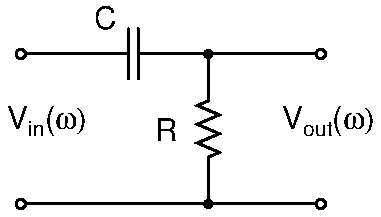
\includegraphics[width=0.25\textwidth]{./schematics/rc_high_pass}
	\begin{parts}
		\part[5]
			What is the transfer function absolute value of this filter at
			$\omega \to 0$ ? \\

			$|G(0)|=$
		\part[5]
			What is the transfer function absolute value of this filter at
			$\omega \to \infty$ ? \\

			$|G(\infty)|=$
		\part[5]
			What is the transfer function absolute value of this filter at
			$\omega = 1/(R C)$ ? \\

			$|G(\frac{1}{R C})|=$
		\part[5]
			What kind of filter is it? (band-pass, low-pass, high-pass,
			band-reject)
		\part[5]
			Find the power dissipated by the Resistor if amplitude of the input
			signal is $V_{in}=2$~V, $R=2$~kOhm, $C=5$~nF, and $\omega = 1/(R C)$.
			\vskip 3in
		\part[5]
			At the same conditions as above.
			Find the power dissipated by the capacitor? 
			\vskip 3in
	\end{parts}

\question
Consider the voltage divider shown  below.\\
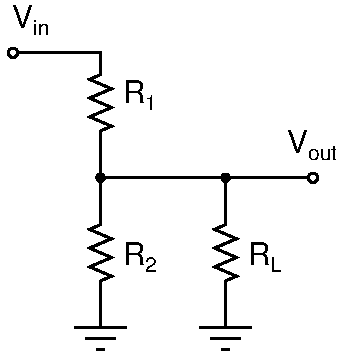
\includegraphics[width=0.25\textwidth]{./schematics/loaded_voltage_divider}
	\begin{parts}
		\part[10]
			What must be the value of the load resistor $R_L$ to ensure maximum power transfer to
			it? If $R_1=4$~kOhm and $R_2=6$~kOhm.
			\vskip 3in
		\part[10]
			At the point of the maximum power transfer to the load resistor. What
			is the value of the current passing through the $R_1$, if $V_{in}=20$~V
			DC?
	\end{parts}
\pagebreak

\question
You are hired as a research assistant for an electronics lab. Your first
assignment is to characterize a black box (which seems to be a power
supply) given to you.  
You know that someone already performed a series of measurements
with this box, and found the voltage drop across several load resistors
connected to the box (see the table below).

\begin{tabular}{|c|c|}
\hline$R_L$	  &  $V_L$ \\ 
\hline
1~kOhm	&  20~V \\
10~Ohm &  1~V \\
\hline
\end{tabular}

	\begin{parts}
		\part[10]
			Find the equivalent  Th\'{e}venin voltage  and resistor of
			this black box. 
			
			\vskip 3in
	\end{parts}

\pagebreak
\question
Your job is to design a low-pass filter with $f_{3dB}=10$~kHz, suitable to
be connected to the source with 200~Ohm internal resistance and capable to
work with loads larger than 1~MOhm.

	\begin{parts}
		\part[5]
			Draw a schematic of the filter which use an {\bf inductor} and resistor.
			\vskip 1in
		\part[5]
			Specify values for the inductor and resistor.
			\vskip 2in
		\part[5]
			Someone who did not read the manual for your filter hooked a 2~kOhm
			load resistor to your filter. Is you filter now high-pass or low-pass one?
			What is the new $f_{3dB}$ frequency?
			\vskip 3in
	\end{parts}

\hide{
\question
Design a band-pass filter  which will pass frequency between 10kHz and
100kHz, with $|G| \ge  0.75$. This filter should attenuate frequencies of
100~Hz and 10~MHz by at least 20~dB. Use only resistors and capacitors.
Assume that you will connect this filter to a signal generator with
an output impedance of 50~Ohm and to a 1~MOhm load resistor.
	\begin{parts}
		\part[5]
			Draw the schematic of the filter
			\vskip 2in

		\part[5]
		Where would you put the low-pass 3~dB point? Why?
		\vskip 1in

		\pagebreak
		\part[5]
		Where would you put the high-pass 3~dB point? Why?
		\vskip 1in

		\part[5]
		Sketch the magnitude of transfer function vs frequency in logarithmic
		scale (G must be in dB).
		\vskip 2in

		\part[10]
		Provide values for resistors and capacitors.
		\vskip 2in
			
		\part[5]
		Which part of the filter can you disregard in your
		calculation at the frequency $f=1000$~MHz? Show a simplified but equivalent
		schematic at this frequency range.
		\vskip 2in

		\part[5]
		What is the approximate value of $G$ measured in dB at
		$f=1000$~MHz. 
	\end{parts}
}

\hide{
\pagebreak
\question
Consider the circuit shown  below.\\
			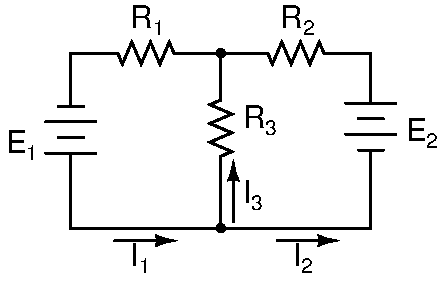
\includegraphics[width=0.45\textwidth]{./schematics/two_loops}
	
	\begin{parts}
		\part[10]
			Using Kirchhoff's laws write down {\bf symbolically} the full set of equation 
			which allows you to find all unknown currents, provided that
			you know all values for resistors and batteries EMF.
			\vskip 2in
		\part[10]
			If $R_1=10$~kOhm, $R_2=5$~kOhm, $R_3=1$~kOhm, $E_1=10$~V, and
			$E_2=5$~V.
			Find the currents $I_1, I_2$ and $I_3$.
			\vskip 3in
		\part[5]
			If resistors remain the same as before but $E_1$ and $E_2$ are
			doubled. What is the new value of $I_1$?
	\end{parts}
	}

\pagebreak
\question
Your experiment apparatus generates useful signal at frequency $f_s = 10$~kHz 
with amplitude voltage $V_s=.2$~V, unfortunately extremely strong
noise couples at frequency $f_n=0.1$~kHz with amplitude $V_n=10$~V.

During this problem you can use approximations and simplified transfer
function representation.

	\begin{parts}
		\part[5]
			What is the signal to noise ration (SNR) coming from the apparatus.
			\vskip 1in
		\part[5]
			In a rush to improve quality of the signal (i.e. SNR) you searched
			through the lab and find a high-pass filter with $f_{3dB} = 2$~Hz.

			What is the SNR at the output of this filter (use linear scale
			not dB to present your answer)? Is it a good filter for the job?
			\vskip 2in
		\part[10]
			If it up to you to design a filter, what kind of filters would you
			use? Where would you place the
			$f_{3dB}$ of your filter?  Draw a schematic of your filter. What is
			the SNR after your filter?
			\vskip 3in
		\part[5]
			If you are not concern about attenuation of the useful signal, what
			is the maximum possible SNR improvement with a single 
			filter? Give it as a ratio of (SNR after)/(SNR before). You can use
			dB if it suits you.
	\end{parts}

\end{questions}
\end{document}

% vim:fdm=marker tabstop=2 shiftwidth=2
